\chapter{Persistence}
In the world of data we rarely have a topological description of the space our dataset lives in. At most, we could consider a set of data points as having the discrete topology but that is not very informative. What if there is an underlying topological space with a non-trivial topology? If so, figuring out properties of this space could provide us with indications of how the data is related \textit{globally}. Consider for example the points sampled from an annulus in Figure \ref{annulus:points}.

\begin{figure}[ht]
  \centering
  \begin{subfigure}[t]{.5\linewidth}
    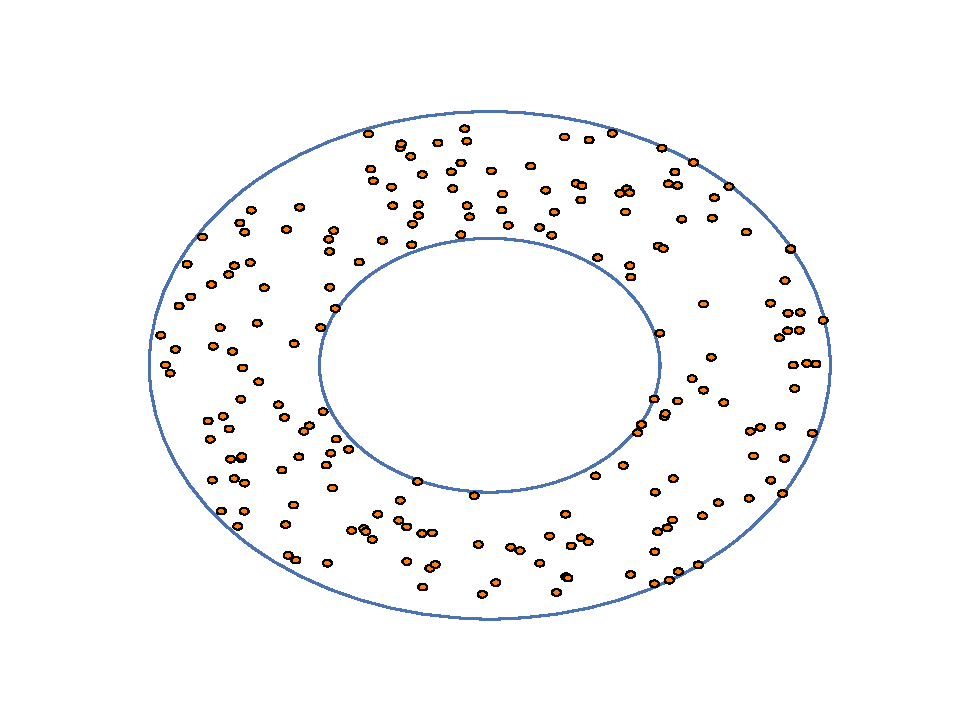
\includegraphics[scale=.5]{annulus.pdf}
    \caption{\label{annulus:points}}
 \end{subfigure}%
  \begin{subfigure}[t]{.5\linewidth}
    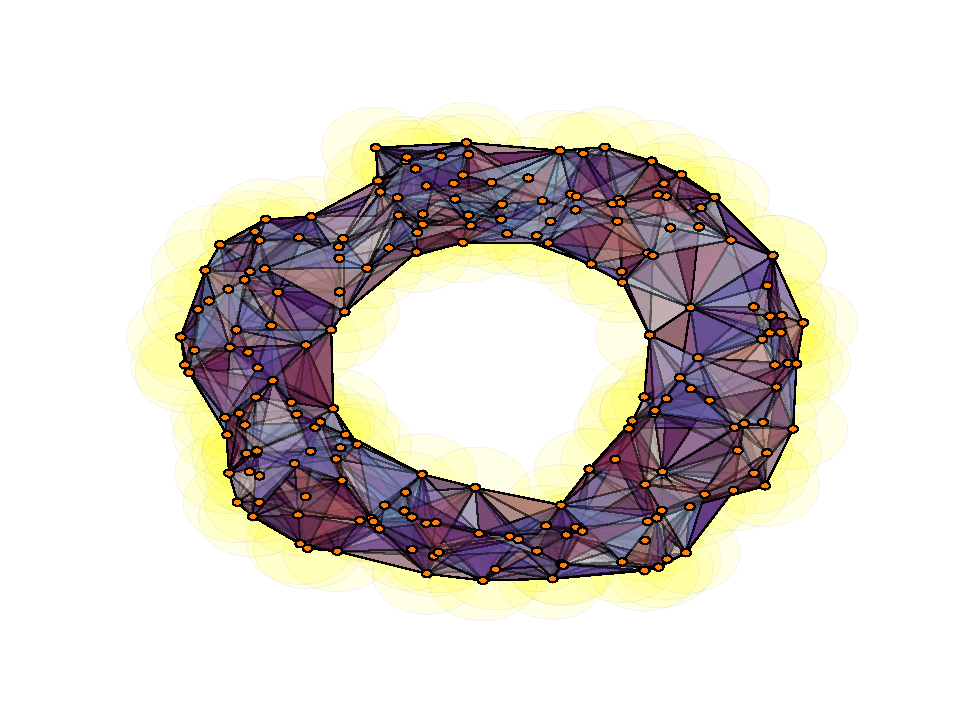
\includegraphics[scale=.5]{annulus_rips.pdf}
    \caption{\label{annulus:imposed}}
 \end{subfigure}
  \caption{\label{annulus} Imposing a simplicial complex \textbf{(b)} on data sampled from an annulus \textbf{(a)}.}
\end{figure}

If we were ignorant of the fact that the underlying space has a the shape of an annulus, which is the situation we more often than not would have in a real-world scenario, being able to deduce the topological properties of this space would tell us that data only lies around a hole. This is where persistent homology comes in, a way of approximating the homology of a space without anything other than the data itself.

The basic principle is quite simple. Using the theory of simplicial homology we can impose a simplicial complex on our dataset as in Figure \ref{annulus:imposed}. A natural way of doing this is defining some form of measure of distance on our data-set, such that when samples are sufficiently close to each other we say they belong to the same simplex.

However, there is a problem with the idea in its naive form. How large is ``sufficiently close''? If we use too large of a distance we end up with all points in a single simplex and retrieve no valuable homological information. On the other hand, if the distance is too small we end up with a simplicial complex with very few connections between vertices and this too could prove uninformative. As we will see, persistent homology circumvents this problem by simply considering \textit{all} possible distances and encoding the homology of the resulting simplicial complexes in a single mathematical object.
% First we need to recall the definition of a homotopy. A homotopy between to continuous maps $f,g$ is another continous map $H: X \times [0,1] \to Y$ such that $H(-,0) = f$ and $H(-,1) = g$. This defines an equivalence relation and we say that $f \simeq g$ meaning that $f$ is homotopy equivalent to $g$.

% We say two topological spaces $X,Y$ are homotopy equivalent, and hence overloading the meaning of this expression, when there exists continuous maps $f: X \to Y$ and $g: Y \to X$ such that $g \circ f \simeq id_{X}$  and $f \circ g \simeq id_{Y}$. This gives an equivalence relation on topological spaces and we write $X \simeq Y$ to mean that they have the same homotopy type.

% After this brief detour we can now look at nerves. We define the nerve of a finite collection of sets to be
% \[nrv(K) = \{ X \subseteq K \mid \bigcap X \neq \emptyset \}\]

% Nerve theorem. Let $F$ be a finite collection of closed convex sets in Euclidean space. Then the nerve of F and the union of the sets in F have the same homotopy type.

\section{Endowing a space with a complex}
A data-set can often be considered as a set of points in Euclidean space. A natural way of endowing a space of points in $\mathbb{R}^{n}$ with a simplicial structure is the following construction.
\begin{definition}[{\cite[p. ~72]{edels}}]
For a family of points $X=\{x_{\alpha}\}_{\alpha}$ in some Euclidean space $\mathbb{R}^{n}$ the \textbf{Čech complex}
$Č_{\epsilon}$ is given by the abstract simplicial complex whose $k$-simplices are given by a subfamily of $k+1$ points $\{x_{\alpha_{i}}\}$ such that \[\bigcap^{k}_{i=0} B_{\epsilon/2}(x_{\alpha_{i}}) \neq \emptyset\] where $B_{r}(x)$ is the closed ball of radius $r$ centered at $x$.
\end{definition}
The Čech complex is a special case of something called the nerve of a topological space, which guarantees that it has the same homology modules as the union of balls centered at the points \cite[p. ~71]{edels}.

However, the Čech complex is for practical purposes not feasible to compute \cite{ghirst}. The reason being that we need to keep the entire simplicial complex in memory and this can be quite large.

A sort of compromise is the Vietoris-Rips complex as seen in Figure \ref{manyrips}. This complex is a simplification where we do not look for points in common between all balls, but rather say that if $k+1$ have balls that intersect \textit{pairwise} they form a $k$-simplex.

\begin{figure}
  \centering
  \begin{subfigure}[t]{.5\linewidth}
    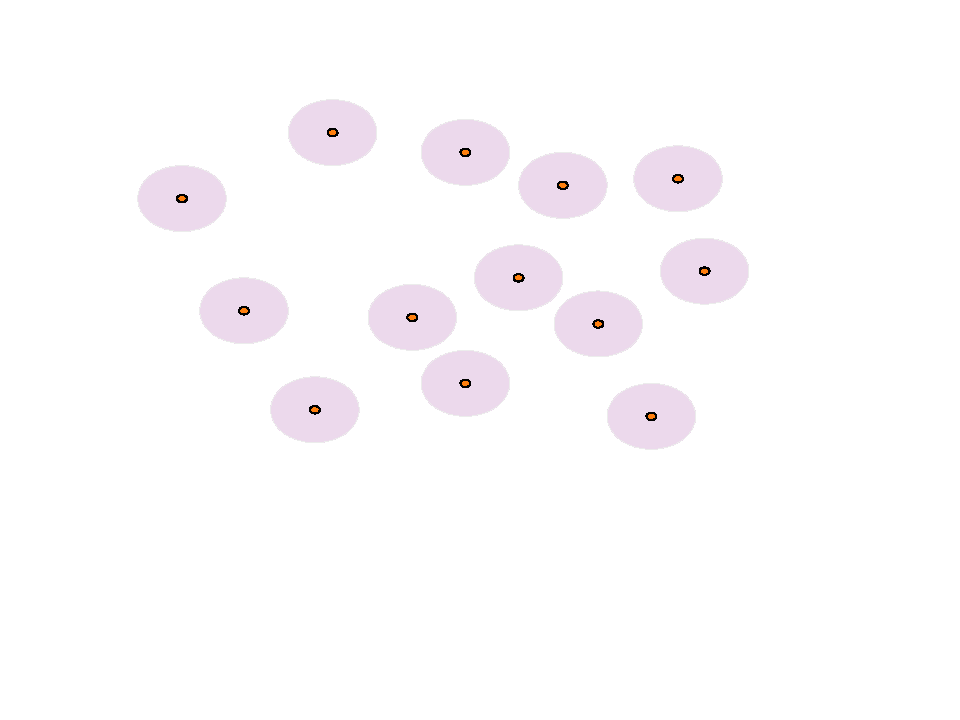
\includegraphics[scale=.5]{rips_eps=01.pdf}
    \caption{$\epsilon=0.1$}
 \end{subfigure}%
  \begin{subfigure}[t]{.5\linewidth}
    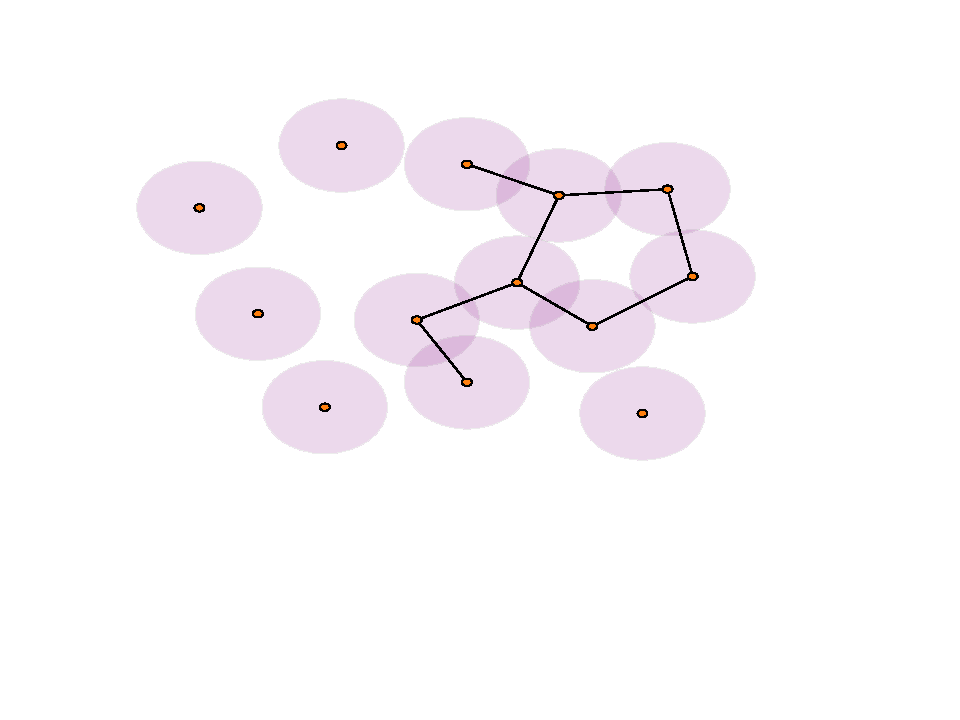
\includegraphics[scale=.5]{rips_eps=015.pdf}
    \caption{$\epsilon=0.15$}
 \end{subfigure}
  \begin{subfigure}[b]{.49\linewidth}
    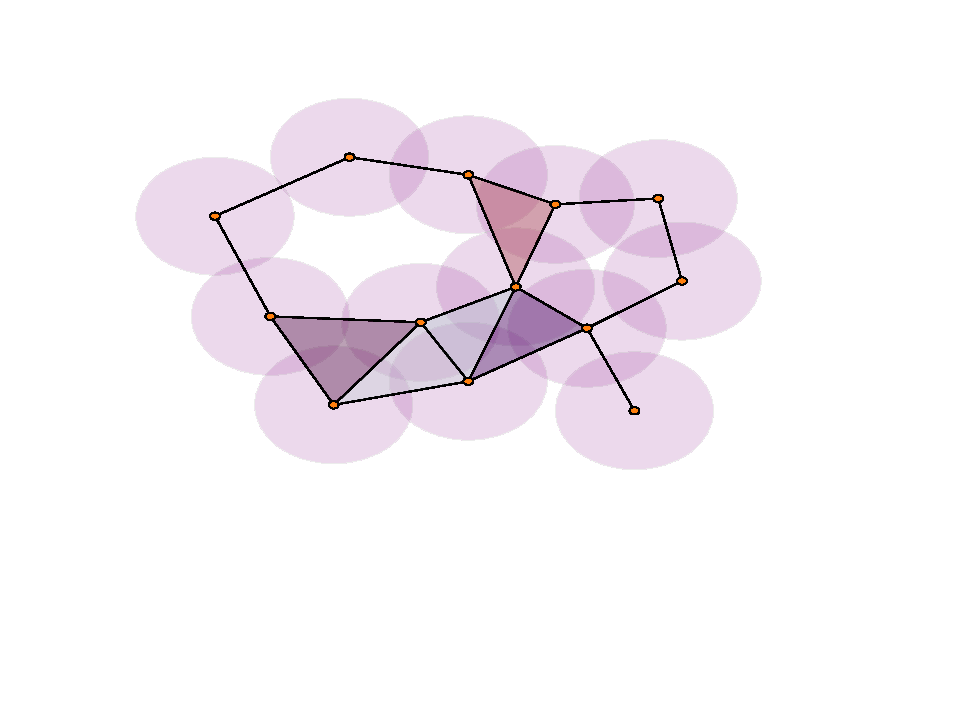
\includegraphics[scale=.5]{rips_eps=02.pdf}
    \caption{$\epsilon=0.2$}
 \end{subfigure}
  \begin{subfigure}[b]{.5\linewidth}
    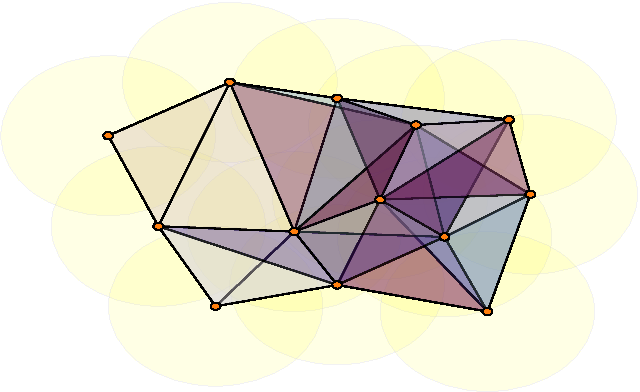
\includegraphics[scale=.5]{rips_eps=03.pdf}
    \caption{$\epsilon=0.3$}
 \end{subfigure}
 \caption{The Vietoris-Rips complex at different $\epsilon$-values.}
 \label{manyrips}
\end{figure}
\begin{definition}[Vietoris-Rips complex]
For a given selection of points $\{x_{\alpha}\}$ in some Euclidean space $\mathbb{R}^{n}$ the Vietoris-Rips complex $R_{\epsilon}$ is the abstract simplicial complex whose $k$-simplices are given by $k+1$ points which are pairwise at most $\epsilon$ apart.
\end{definition}

The Vietoris-Rips complex does not come with the same guarantee of fidelity to the underlying space as the Čech complex does. However, it is entirely defined by the vertices and the edges of the simplicial complex, allowing it to be stored as a graph.

Given a monotonically increasing sequence of real numbers $(\epsilon_{i})^{n}_{i}$ we can for each $\epsilon_{i}$ associate to a finite set of points $X$ the Vietoris-Rips complex $R_{\epsilon_{i}}$. Then as illustrated in Figure \ref{manyrips} we have inclusions
\begin{center}
\begin{tikzcd}
R_{\epsilon_1} \arrow[hookrightarrow]{r}{\iota} & R_{\epsilon_2} \arrow[hookrightarrow]{r}{\iota} & \dots \arrow[hookrightarrow]{r}{\iota} & R_{\epsilon_{n-1}} \arrow[hookrightarrow]{r}{\iota} & R_{\epsilon_n}.
\end{tikzcd}
\end{center}
For $i<j$ the inclusion $\iota: R_{\epsilon_i} \to R_{\epsilon_{j}}$ induces a map $\iota_{*}: H_{k}(R_{\epsilon_{i}}) \to H_{k}(R_{\epsilon_j})$ and the image of this map tell us which equivalence classes in $H_{k}$ survive when going from $R_{\epsilon_{i}}$ to $R_{\epsilon_{j}}$, in other words the homological features that persist going from resolution $\epsilon_{i}$ to resolution $\epsilon_{j}$ in the Vietoris-Rips construction. The following result then lends some credibility to the Vietoris-Rips complex through its relationship with the Čech complex.
\begin{lemma}[{\cite[Vietoris-Rips Lemma, p. ~74]{edels}}]
  Given $\epsilon > 0$ there is a chain of inclusions
  \[R_{\epsilon} \hookrightarrow C_{\epsilon \sqrt{2}} \hookrightarrow R_{\epsilon \sqrt{2}}\]
\end{lemma}
Hence, any cycle that persists through the induced map $H_{k}(R_{\epsilon}) \to H_{k}(R_{\epsilon'})$ for $\epsilon'  \geq \sqrt{2} \epsilon$ is also present in the Čech complex $Č_{\epsilon}'$.

The insight that the homological features that persist tell us more than the individual homology groups themselves are central to the idea of persistent homology. Before we give the formal definition of persistent homology we must first generalize the concept of endowing a space with a complex.

\begin{definition}
A \textbf{filtration} $F$ of a simplicial (or cubical) complex $K$ is a totally ordered set of subcomplexes $K^{i}  \subseteq K$ for $i \in \mathbb{N}$ such that if $i \leq j$ then $K^{i} \subseteq K^{j}$.
\end{definition}

Note that the Čech and Vietoris-Rips constructions over a sequence of resolutions are two instances of filtrations, but with this definition we are not restricted to them alone. With this definition in place, we can state the formal definition of persistent homology.

\begin{definition}\label{phfirstdef}
  For $p > 0$ the \textbf{$p$-persistent $k$th homology module} of filtration $F$ is given as
  \[H^{i,p}_{k} = Z^{i}_{k}/(B^{{i+p}}_{k} \cap Z^{i}_{k})\]
  where $Z^{i}_{k},B^{i}_{k}$ are the cycle and boundary modules of the resulting chain complexes $C_*(F_{i})$
\end{definition}
This module is well-defined since the inclusion $K^{i} \hookrightarrow K^{i+p}$ induces inclusions $C^{i}_{k} \hookrightarrow C_{k}^{i+p}$ hence we have inclusions $Z^{i}_{k} \hookrightarrow C^{i}_{k} \hookrightarrow C_{k}^{i+p}$ and so $Z^{i}_{k}$ is a submodule of $C^{i+p}_{k}$. Furthermore, it captures precisely what we have been alluding to earlier: the $p$ persistent homology modules are exactly the equivalence classes that survive up to some filtration $p$.


\section{Persistence Module}
While Definition \ref{phfirstdef} serves as a sufficient framework for persistent homology, it is still particular in the sense that it is stated in terms of filtrations and chain complexes arising from them. It is possible to make the notion of persistence even more general which allows us to understand its algebraic structure. This does not mean that we should entirely discard our anchoring of persistent homology in the realm of simplicial complexes, as it relates closely to how we will do persistent homology in practice, but rather we should let this more abstract approach serve as the theoretical underpinning which opens up the possibility of other types of approximation of data than simplicial complexes.

\begin{definition}[{\cite[p. ~2]{weibel1994}}]
  Let $C_{*},D_{*}$ be chain complexes over some ring $R$. A \textbf{chain map} $u: C_{*} \to D_{*}$ is a family of $R$-module homomorphisms $u_{k}: C_{k} \to D_{k}$ such that the following diagram commutes
  \begin{center}
% https://tikzcd.yichuanshen.de/#N4Igdg9gJgpgziAXAbVABwnAlgFyxMJZARgBoAGAXVJADcBDAGwFcYkQBhAfWAGsBqYgF8QQ0uky58hFACYK1Ok1btuvUeJAZseAkQDMCmgxZtEnHrwC0wjRJ3SiZYopMrzAEUuCRY+1L05UhdjZTMQL3U-LUldGWRDEKVTdi8+G19NbQD48iNk9xAAHSKoCBwEaOy4ojykt3CSsoq7GIdA5AAWfIb2JvLKrNjHFG76sL7SgdFFGCgAc3giUAAzACcIAFskADYaHAgkPILGorR6Nbwmb1lM1Y3txGODpEMT9mZvW2j1raQAdn2h0Qb165hK50uWGufH4t1av0ez2BZHe4LOFyujC+dxAiKQqJeiHkaOKGKhMN4uPxIKBSG6pIhmOh2Nh300NIZRIArKEUujIViuFEOQ8kCSeXzCp90uz7n9iXTEAAOKWnQUsywZBFixC8kBEgCcasmGsp2p+usJwIZYJAnyilCEQA
\begin{tikzcd}
\dots \arrow[r, "\partial_{k+2}"] & C_{k+1} \arrow[d, "u_{k+1}"] \arrow[r, "\partial_{k+1}"] & C_k \arrow[r, "\partial_{k}"] \arrow[d, "u_k"] & C_{k-1} \arrow[d, "u_{k-1}"] \arrow[r, "\partial_{k-1}"] & \dots \\
\dots \arrow[r, "\partial_{k+2}"] & D_{k+1} \arrow[r, "\partial_{k+1}"]                      & D_k \arrow[r, "\partial_k"]                    & D_{k-1} \arrow[r, "\partial_{k-1}"]                      & \dots
\end{tikzcd}
  \end{center}
\end{definition}

\begin{definition}
  A \textbf{persistence complex} is a family of chain complexes $C^{i}_{*}$ together with chain maps $\iota^{i}: C^{i} \to C^{i+1}$ that go between them in the following way
% https://tikzcd.yichuanshen.de/#N4Igdg9gJgpgziAXAbVABwnAlgFyxMJZARgBpiBdUkANwEMAbAVxiRAGkA9YLAXwH1gAawDUxXiF6l0mXPkIoyAJiq1GLNlyyChEqTOx4CRJeVX1mrRB25YxA4fcnSQGQ-JOkV1Cxutceex09Fzc5YxQABjMfdSsQAB0EqAgcBH1XWSMFZGjvNUs2JJS05wNwnLJI8ziihJoS9NCsjxRTatjC6ySG1Kby7KIAZhiCv0TkvrLM9wjkEfzfeOKpjLDBxVIhmq6J3tK1lrnTbc7xnsbJVRgoAHN4IlAAMwAnCABbJDIQHAgkEZ+dCwDDYAAsIBAhCAzssEvgcHR+Fhpq8Pkhoj8-ohvgw6AAjGAMAAKRwUIAYMCeOGhY1haDoLzwjB0TgyqM+iFMmP+MLq9MZWGZjnEKLeHIxvyQXIRwLBEKh1FxBOJpLYFKpNKWdXhdE4yLZYqQABZqJLEBKgSDrODIZrat04alETwALQig1oxAAVlNWO+MqtIBtCtp2qdgiwbpCz0NnN9SAAHKbLXLbbyHTqI6yXOyedzEABOZOy63yu27JKZwLunOxgBs8fN6Ym-KZDBZSmjIFziAA7I2uVqHa3Be3HJ3RZ7-X6MUOWwy2-woR6OQCzcRvnOkiPmcuKLwgA
\begin{center}
\begin{tikzcd}
                                     & \vdots \arrow[d, "\partial_{k+2}"]                                 & \vdots \arrow[d, "\partial_{k+2}"]                                       &       \\
\dots \arrow[r, "\iota^{i-1}", hook] & C^{i}_{k+1} \arrow[d, "\partial_{k+1}"] \arrow[r, "\iota^i", hook] & C^{i+1}_{k+1} \arrow[d, "\partial_{k+1}"] \arrow[r, "\iota^{i+1}", hook] & \dots \\
\dots \arrow[r, "\iota^{i-1}", hook] & C^i_{k} \arrow[r, "\iota^i", hook] \arrow[d, "\partial_k"]         & C^{i+1}_{k} \arrow[r, "\iota^{i+1}", hook] \arrow[d, "\partial_k"]       & \dots \\
                                     & \vdots                                                             & \vdots                                                                   &
\end{tikzcd}
\end{center}
\end{definition}

% \begin{definition}
% Given a persistence complex we define the $(i,j)$-persistent homology $H_{*}^{{i\to j}}(C)$, where $i < j$, to be the image of the induced homomorphism on homology $\iota_{*}: H_{*}(C_{*}^{i}) \to H_{*}(C_{*}^{j})$.
% \end{definition}
\begin{definition}[\cite{Zomorodian2005}]
  A \textbf{persistence module} $M$ is a family of $R$-modules $M^{k}$ together with module homomorphisms $\phi: M^{k} \to M^{k+1}$.
\end{definition}
With the definition of the persistence module we arrive at an alternate definition of persistent homology, the persistent homology of a persistence complex.
\begin{definition}\label{altdef} For $p>0$ the $p$-persistent homology of a persistence complex $(C_{*}, \iota)$ is denoted $H^{p}_{*}$ and is defined to be the images of the induced homomorphisms $\iota^{p-1}_{*} \circ \iota^{p-2}_{*} \circ \dots \circ \iota^{i}_{*}: H_{*}(C_{*}^{i}) \to H_{*}(C^{p}_{*})$.
\end{definition}
In the light of this definition, we see that the $p$-persistent homology of a persistence complex is a persistence module where the module homomorphisms $\phi$ are the maps induced by the chain maps $\iota: C^{i}_{*} \to C_{*}^{i+1}$. The objects given in definitions \ref{phfirstdef} and \ref{altdef} are in fact isomorphic.
\begin{lemma}
Let $\iota^{i,p}_k: H^{i}_{k} \to H^{p}_{k}$ be the module homomorphism that takes a class in $H^{i}$ to the class which contains that class in $H^{p}$. Then $Im (\iota^{i,p}_{k}) \simeq H^{p}_{k}$.
\end{lemma}
\begin{proof}
  Note that the kernel of $\iota^{{i,p}}$ are exactly those classes of cycles which become boundaries at some index $i,i+1,\dots,p$, hence $\ker (\iota^{i,p}) = (B^{i+p} \cap Z^{i})$. So by the first isomorphism theorem for modules we get that
  \[ Im (\iota^{i,p}) \simeq H^{i}_{k} / \ker(\iota^{i,p}) \simeq H^{i}_{k} / (B^{i+p} \cap Z_{k}^{i}) \simeq (Z^{i}_{k}/B^{i}_{k})/(B^{i+p}_{k}\cap Z^{i}_{k}) \simeq H^{i,p}_{k} \]
  where last isomorphism follows from the fact that $B^{i}_{k} \subseteq B_{k}^{i+p} \cap Z^{i}_{k}$.
\end{proof}

\begin{definition}[\cite{Zomorodian2005}]
We say a persistence module $(M^{k}, \phi^{k})$ is of \textbf{finite type} if each component $M^{k}_{n}$ is a finitely generated $R$-module and the maps $\phi^{k}$ are isomorphisms for $k \geq N$ for some integer $N$.
\end{definition}

When we start with a finite simplicial complex $K$ we get that $C_{*}(K)$ is consists of finitely generated $R$-modules, since the number of simplices in each dimension is finite, and so the resuling persistence complex and persistence modules are of finite type.

The most important theoretic result is just around the corner, but before that we need to recall some definitions regarding graded rings and modules.

\begin{definition}
  Let $R$ be a ring. We say $R$ is a \textbf{graded ring} if it can be decomposed as
  \[ R = \bigoplus_{i} R_{i}\]
\end{definition}
Note that given a ring $R$ the polynomial ring $R[x]$ is always a graded ring, since it can be decomposed into $R[x] = Rx^{0} \oplus Rx^{1} \oplus \dots$

\begin{definition}
A non-zero element $r$ in a graded ring $R$ is said to be homogenous of degree $n$ if $r \in R_{n}$ and $r \not \in R_{j}$ for all $j \neq n$.
\end{definition}

In other words, the homogenous elements of a graded ring are those elements that are contained to a single component. Adding elements from different components give us elements that are not homogenous.
\begin{definition}
  Let $R = \bigoplus_{{i}} R_{i}$ be a graded ring and $M$ a left $R-module$. We say that $M$ is a \textbf{graded $R$-module} if
  \[M = \bigoplus_{i} M_{i} \]
  where $M_{i}$ are submodules of $M$, such that $R_{i}M_{j} \subseteq M_{i+j}$.
\end{definition}

Most of the ordinary algebraic constructions on modules hold for graded modules as well. The only additional requirement is that they preserve homogenous elements in the obvious way. For example, a morphism of graded modules is a morphism of modules such that it preserves degree. In other words, a morphism takes an element in a graded module of degree $n$ to an element in another graded module of degree $n$. Similarly, a graded submodule of a module is simply a graded module such that each component is a submodule of the corresponding module.

We can now see that if we have a persistence module $M$ over some ring $R$ and we give $R$ a graded structure by considering $R[t]$ then a graded module structure on $M$ is given by
\[ \alpha(M) = \bigoplus^{\infty}_{k=0} M^{k}\]
The action $t^{p}$ sends $M^{k} \to M^{k+p}$ by $p$ repeated applications of $t$, in other words $t$ shifts the elements up in the graduation by its power
\[ t \cdot (m^{0}, m^{1}, m^{2}, \dots  ) = (0, \phi^{0}(m^{0}), \phi^{1}(m^{1}),\phi^{2}(m^{2}),\dots) \]
and so we get that $R[t]_{p}M^{k} = Rt^{p}M^{k} \subseteq M^{k+p}$ which satisfies the condition we gave in our definition of a graded module.

The map $\alpha$ is actually an isomorphism between the category of persistence modules and graded modules \cite{ghirst}. Hence, for ease of notation we will simply consider a persistence module to be a graded module when necessary. This gives us a lot for free: we do not have to be afraid of taking quotients or direct sums of persistence modules as we know what objects they correspond to in the category of graded modules. For example, we write $H$ for the direct sum of the persistence modules $H_{k}$ and similarly we write $C$ for the persistence complex given by the sum of the persistence modules $C_{k}$.

We now arrive at the result which fully characterizes the algebraic structure of persistent homology. This result comes with a caveat, namely that it only characterizes persistence modules of finite type over a field. The more general problem is under the functor $\alpha$ equivalent to characterizing graded $\mathcal{R}[t]$ modules over an arbitrary ring $\mathcal{R}$, which is known to be a hard problem \cite{ghirst}.
\begin{theorem}[{\cite{Zomorodian2005}}] \label{structurethm1}
  For a persistence module $M$ of \textit{finite type} over a field $\mathbb{F}$,
  \[M \cong \bigoplus_{i} t^{p_{i}} \cdot \mathbb{F}[t] \oplus (\bigoplus_{j} (t^{r_{j}} \cdot \mathbb{F}[t]) / (t^{s_{j}}) \]

\end{theorem}

While the restriction to a field $\mathbb{F}$ somewhat limits the usefulness of the decomposition, we often in practice prefer working in $\mathbb{Z}_{2}$ due to computational aspects and hence in most cases it poses no real problem.

The proof of Theorem \ref{structurethm1} is constructive and ultimately leads to an algorithm for computing persistent homology in terms of linear algebra. Hence, persistent homology is computable in practical applications even for large data-sets. Due to the intimate relation between the proof and the computational aspects we will give it an appropriate treatment in the next section.

Theorem \ref{structurethm1} has an intuitive explanation in terms of filtrations: when $M$ is the persistent homology $H$ given by some filtration $F$, the free part consists of generators which appear in the subcomplex $F_{p_{i}}$ and continue to exist for all future filtrations. The torsional part consists of generators which appear at in the subcomplex $F_{r_{j}}$ and disappear in  $F_{r_{j}+s_{j}}$. Furthermore, the decomposition provides the $p$-persistent homology for all $p$ and so we circumvent the problem of having to choose an optimal step of the filtration of which to compute homology.

We can make this association of the decomposition of a persistence module with intervals more precise through the following definitions.

\begin{definition}
  For a persistence module $M$ as in Theorem \ref{structurethm1} we associate the interval $(i,j) \in \mathbb{N}\cup \{\infty\}$ to ${M}$ as
  \[Q(i,j):= t^{i} \cdot \mathbb{F}[t]/t^{{j-i}},\]

  \[Q(i,\infty):= t^{i} \cdot \mathbb{F}[t].\]
  Furthermore, given a set of intervals $S = \{(i_{0},j_{0}),\dots,(i_{n},j_{n})\}$ we say that
  \[Q(S) := \bigoplus_{k} Q(i_{k},j_{k}).\]
  The \textbf{barcode} $\mathbf{B_{M}}$ is the multiset of intervals $Q^{-1}(M)$.
\end{definition}


In the obvious way, $Q$ is a bijection which maps each summand in the decomposition of a persistence module to an interval. This gives us a correspondence between infinite intervals and generators of the free part and finite intervals and generators of the torsional part.


\section{Proof of the Structure Theorem}
As promised we will now derive the connection between linear algebra and persistence modules. A key observation is that for every (graded) module $M$ there is an exact sequence
\[ K \to G \to M \to 0\]
where $G$ is the free module on the generators of $M$ and $K$ is the kernel of the projection onto $M$. We call this the \textbf{presentation} of $M$ and it follows by the first isomorphism theorem we have an isomorphism $M \cong G/\text{im f}$, and hence we can characterize $M$ by only knowing $K,G$ and $f$.
\begin{lemma}[{\cite[Theorem 7]{skraba}}]
  When $M$ is a persistence module of finite type the presentation of $M$ becomes a short exact sequence
  \[ 0 \to K \to G \to M \to 0\]
  where $K$ is also free. We call this the \textbf{free presentation} of $M$.
\end{lemma}
When $K,G$ are free the map $f$ is a map $\mathbb{F}[t]^{n} \to \mathbb{F}[t]^{m}$, in other words it can for a given choice of bases be represented by a matrix in $\mathbb{F}[t]^{n \times m}$ which we call a \textbf{presentation matrix} of $M$. This is the vital connection between persistence modules and linear algebra. By reducing this matrix, much like in the process of Gaussian elimination, we end up with a matrix that describes compatible bases in $K$ and $G$. Then $M$ is generated by the basis in $G$ with relations given by the basis in $K$.

\begin{definition}
A matrix with coefficients in $\mathbb{F}[t]$ is in \textbf{graded Smith normal} if its only non-zero entries are on the (possibly permuted) diagonal and these entries are homogeneous elements.
\end{definition}

We will now describe an algorithm for computing the graded Smith normal form. Since the resulting matrix will consist of linearily independent columns and rows they define a basis for the column and row space.

\begin{algorithm}
\caption{Reduction to graded Smith normal form \cite{skraba, Zomorodian2005}}\label{smith}
\begin{algorithmic}[1]
  \State \textbf{Input:} Matrix $ \in \mathbb{F}[t]^{n \times m}$ with homogeneous entries with columns and rows sorted in order of ascending degree.
  \State \textbf{Returns:} Matrix $ \in \mathbb{F}[t]^{n \times m}$ in graded Smith normal form with columns and rows sorted in order of ascending degree.
  \For{$i < m, j < n$}
  \State Eliminate all entries \textit{rightwards} by column additions in row $i$.
  \State Eliminate all entries \textit{upwards} by row additions in column $j$.
\end{algorithmic}
\end{algorithm}
\begin{proof}(\textbf{Correctness of Algorithm 1.})
  To show the correctness of the algorithm it suffices to show that we can eliminate entries and that such elimination does not change the degrees of the homogenous basis elements given by the rows and columns.

  Suppose we wish to eliminate some entry in row $j$ with an element in row $i$. This implies that $ i > j$ by the algorithm itself. Let the entries be denoted $a_{i}= c \cdot t^{r_{i}}$ and $b_{j} = d \cdot t^{s_{j}}$ respectively. Since the columns and rows are chosen to be homogeneous, we know that they can be written this way. The matrix is sorted in ascending degree order in both rows and columns, which implies that $\deg(a_{i}) \leq \deg(b_{j})$, hence we can always eliminate $b_{j}$ by adding $t^{s_{j}-r_{i}} \frac{-d}{c} \cdot a_{i}$. Furthermore, if $\gamma_{i},\gamma_{j}$ are the basis elements of rows $i,j$ then we know from linear algebra that the addition causes a change of basis $\gamma'_{i}:=\gamma_{i}-t^{s_{j}-r_{i}} \frac{-d}{c} \cdot \gamma_{j}$. We get that $\deg(\gamma'_{i})=\max\{\deg(\gamma_{i}), (s_{j}-r_{i}+\deg(\gamma_{j})\}$, but since $a_{i},b_{j}$ are entries of the same homogeneous column this implies that $r_{i} + \deg(\gamma_{i}) = s_{j} + \deg(\gamma_{j})$, hence $\deg(\gamma'_{i}) = \deg(\gamma_{i})$. An identical argument holds for if we wish to eliminate by column additions, with the exception that it is $\gamma_{j}$ that changes basis.
\end{proof}
When a presentation matrix of $M$ is put into graded Smith normal form by Algorithm 1 it gives us compatible bases for $K$ and $G$ and the isomorphism becomes \[M\cong \text{zero rows of matrix}/\text{non-zero rows of matrix times their entry}.\]
We are now ready to prove Theorem \ref{structurethm1}.

\begin{proof}
  The module $M$ is of finite type so it has a presentation matrix $P$. By reducing $P$ to graded Smith normal form with Algorithm 1 we get a matrix $P'$. Since $M \cong G/K$ by the first isomorphism theorem we have that $M$ is generated by the basis elements of $G$ given by the zero rows of $P'$, as these are basis elements which are not hit by the inclusion $K \hookrightarrow G$. Furthermore, the torsional part in the decomposition is given by the non-zero rows which define those basis elements of $K$ which shifted by their entry are killed in $M$. This proves the existence of the decomposition.

  What remains to show is that the decomposition is unique no matter our choice of generators for $G$ and $K$. This actually follows from a much more general result, the Krull-Schmidt Theorem \cite[p. ~115]{jacobson2009basic}, but we will give a proof for our specific situation. Suppose that we have two different decompositions of $M$ that we denote $C,D$. We claim that they are identical up to permutation of components and modulo trivial components. We have homomorphisms
  \[
    f_{ij} := C_{i} \hookrightarrow C \cong M  \cong D  \twoheadrightarrow D_{j},
  \]
  \[
    g_{ij} :=  D_{j} \hookrightarrow D \cong M  \cong C  \twoheadrightarrow C_{i}
  \]
  where the maps are the obvious inclusions and projections from and onto components. Then for at least one pair $i,j$ the homomorphism $f_{ij}$ cannot be the zero map since $\bigoplus_{i,j} g_{ij} \circ f_{ij}: C \to C$ is an automorphism of $C$. But this implies that $f_{ij}$ is an isomorphism $C_{i} \cong D_{j}$ and so the original claim follows by induction.

\end{proof}
Now for explicitly computing persistent homology we have the presentation

\[
  0 \to B \to Z \to H \to 0
\]
and so we could theoretically apply the proof above and get a decomposition of $H$, but this comes with one caveat: to give a presentation matrix of $H$ requires us to first have a basis of $Z$, which we typically do not have. Instead we have the boundary map $\partial: C \to C$ which has as its image $B$ and $Z$ as its kernel. Hence, we must first compute the Smith graded normal form of the map $\partial$ which gives us a compatible basis in both $B$ and $Z$. Then we compute the Smith normal form of the inclusion map $B \to Z$ from which we can derive the barcode $\mathbf{B}_{H}$.

\begin{example}\label{bddreduce}
Consider the filtration given in Figure \ref{filtrationstack}. For simplicity we work in $\mathbb{F}=\mathbb{Z}_{2}$. The persistence complex has basis given by the simplices $v_{0},v_{1},v_{2},v_{12},v_{20},v_{01},v_{03},v_{120}$. We get boundaries the following boundaries by evaluating the boundary map on the basis elements, \[v_{2}+v_{1},t(v_{1})+t^{2}(v_{0}),t(v_{2})+t^{2}(v_{0}),v_{3}+t^{2}v_{0}, t^{2}(v_{12})+t(v_{10})+t(v_{20}).\]
hence we have the following matrix representing the map $\partial$:
\[
  \bordermatrix{
    & v_{0} & v_{1} & v_{2} & v_{3} & v_{12} & v_{20} & v_{01} & v_{03} & v_{120}\cr
    v_{0}  &.&.&.&.&.&t^{2}&t^{2}&t^{2}&.\cr
    v_{1}  &.&.&.&.&1&.&t&.&.\cr
    v_{2}  &.&.&.&.&1&t&.&.&.\cr
    v_{3}  &.&.&.&.&.&.&.&1&.\cr
    v_{12} &.&.&.&.&.&.&.&.&t^{2}\cr
    v_{20} &.&.&.&.&.&.&.&.&t\cr
    v_{01} &.&.&.&.&.&.&.&.&t\cr
    v_{03} &.&.&.&.&.&.&.&.&.\cr
    v_{120}&.&.&.&.&.&.&.&.&.
    }
  \]
  Reducing this matrix to graded Smith normal form while keeping track of basis changes gives us the matrix
%     \[
%       \to
% \bordermatrix{
%     & v_{0} & v_{1} & v_{2} & v_{3} & v_{12}  & v_{20} + tv_{12}& v_{01} & v_{03} & v_{120}\cr
%     v_{0}  &.&.&.&.&.&t^{2}&t^{2}&t^{2}&.\cr
%     v_{1}  &.&.&.&.&1&t&t&.&.\cr
%     v_{2}  &.&.&.&.&1&.&.&.&.\cr
%     v_{3}  &.&.&.&.&.&.&.&1&.\cr
%     v_{12} &.&.&.&.&.&.&.&.&t^{2}\cr
%     v_{20} &.&.&.&.&.&.&.&.&t\cr
%     v_{01} &.&.&.&.&.&.&.&.&t\cr
%     v_{03} &.&.&.&.&.&.&.&.&.\cr
%     v_{120}&.&.&.&.&.&.&.&.&.
%     }
% \]

%     \[
% \bordermatrix{
%     & v_{0} & v_{1} & v_{2} & v_{3} & v_{12} & v_{20}+tv_{12} & v_{01}+v_{20}+tv_{12} & v_{03} & v_{120}\cr
%     v_{0}  &.&.&.&.&.&t^{2}&.&t^{2}&.\cr
%     v_{1}  &.&.&.&.&1&t&.&.&.\cr
%     v_{2}  &.&.&.&.&1&.&.&.&.\cr
%     v_{3}  &.&.&.&.&.&.&.&1&.\cr
%     v_{12} &.&.&.&.&.&.&.&.&t^{2}\cr
%     v_{20} &.&.&.&.&.&.&.&.&t\cr
%     v_{01} &.&.&.&.&.&.&.&.&t\cr
%     v_{03} &.&.&.&.&.&.&.&.&.\cr
%     v_{120}&.&.&.&.&.&.&.&.&.
%     }
%   \]

%     \[
% \bordermatrix{
%     & v_{0} & v_{1} & v_{2} & v_{3} & v_{12} & v_{20}+tv_{12} & v_{01}+v_{20}+tv_{12} & v_{03} & v_{120}\cr
%     v_{0}  &.&.&.&.&.&t^{2}&.&t^{2}&.\cr
%     v_{1}  &.&.&.&.&.&t&.&.&.\cr
%     v_{2}+v_{1}  &.&.&.&.&1&.&.&.&.\cr
%     v_{3}  &.&.&.&.&.&.&.&1&.\cr
%     v_{12} &.&.&.&.&.&.&.&.&t^{2}\cr
%     v_{20} &.&.&.&.&.&.&.&.&t\cr
%     v_{01} &.&.&.&.&.&.&.&.&t\cr
%     v_{03} &.&.&.&.&.&.&.&.&.\cr
%     v_{120}&.&.&.&.&.&.&.&.&.
%     }
%   \]

%     \[
% \bordermatrix{
%     & v_{0} & v_{1} & v_{2} & v_{3} & v_{12} & v_{20}+tv_{12} & v_{01}+v_{20}+tv_{12} & v_{03} & v_{120}\cr
%     v_{0}  &.&.&.&.&.&.&.&t^{2}&.\cr
%     v_{1}+tv_{0}  &.&.&.&.&.&t&.&.&.\cr
%     v_{2}+v_{1}  &.&.&.&.&1&.&.&.&.\cr
%     v_{3}  &.&.&.&.&.&.&.&1&.\cr
%     v_{12} &.&.&.&.&.&.&.&.&t^{2}\cr
%     v_{20} &.&.&.&.&.&.&.&.&t\cr
%     v_{01} &.&.&.&.&.&.&.&.&t\cr
%     v_{03} &.&.&.&.&.&.&.&.&.\cr
%     v_{120}&.&.&.&.&.&.&.&.&.
%     }
%   \]
% \[
% \bordermatrix{
%     & v_{0} & v_{1} & v_{2} & v_{3} & v_{12} & v_{20}+tv_{12} & v_{01}+v_{20}+tv_{12} & v_{03} & v_{120}\cr
%     v_{0}  &.&.&.&.&.&.&.&.&.\cr
%     v_{1}+tv_{0}  &.&.&.&.&.&t&.&.&.\cr
%     v_{2}+v_{1}  &.&.&.&.&1&.&.&.&.\cr
%     v_{3}+t^{2}v_{0}  &.&.&.&.&.&.&.&1&.\cr
%     v_{12} &.&.&.&.&.&.&.&.&t^{2}\cr
%     v_{20} &.&.&.&.&.&.&.&.&t\cr
%     v_{01} &.&.&.&.&.&.&.&.&t\cr
%     v_{03} &.&.&.&.&.&.&.&.&.\cr
%     v_{120}&.&.&.&.&.&.&.&.&.
%     }
%   \]
%     \[
% \bordermatrix{
%     & v_{0} & v_{1} & v_{2} & v_{3} & v_{12} & v_{20}+tv_{12} & v_{01}+v_{20}+tv_{12} & v_{03} & v_{120}\cr
%     v_{0}  &.&.&.&.&.&.&.&.&.\cr
%     v_{1}+tv_{0}  &.&.&.&.&.&t&.&.&.\cr
%     v_{2}+v_{1}  &.&.&.&.&1&.&.&.&.\cr
%     v_{3}+t^{2}v_{0}  &.&.&.&.&.&.&.&1&.\cr
%     v_{12} &.&.&.&.&.&.&.&.&.\cr
%     v_{20} &.&.&.&.&.&.&.&.&t\cr
%     v_{01}+tv_{12} &.&.&.&.&.&.&.&.&t\cr
%     v_{03} &.&.&.&.&.&.&.&.&.\cr
%     v_{120}&.&.&.&.&.&.&.&.&.
%     }
%   \]

    \[
\bordermatrix{
    & v_{0} & v_{1} & v_{2} & v_{3} & v_{12} & v_{20}+tv_{12} & v_{01}+v_{20}+tv_{12} & v_{03} & v_{120}\cr
    v_{0}  &.&.&.&.&.&.&.&.&.\cr
    v_{1}+tv_{0}  &.&.&.&.&.&t&.&.&.\cr
    v_{2}+v_{1}  &.&.&.&.&1&.&.&.&.\cr
    v_{3}+t^{2}v_{0}  &.&.&.&.&.&.&.&1&.\cr
    v_{12} &.&.&.&.&.&.&.&.&.\cr
    v_{20} &.&.&.&.&.&.&.&.&.\cr
    v_{01}+tv_{12}+v_{20} &.&.&.&.&.&.&.&.&t\cr
    v_{03} &.&.&.&.&.&.&.&.&.\cr
    v_{120}&.&.&.&.&.&.&.&.&.
    }
  \]
  From the reduction to normal form we can read off a basis for $Z$ given by the zero columns and the basis of $B$ given by the non-zero rows together with their non-zero entry. This gives us a presentation matrix of $H$ from the inclusion $B \hookrightarrow Z$

  \[
    \bordermatrix{& v_{2}+v_{1} & tv_{1}+t^{2}v_{0} & v_{3}+t^{2}v_{0} & tv_{01}+t^{2}v_{12}+tv_{20} \cr
      v_{0} & . & t^{2} & t^{2} & . \cr
      v_{1} & 1 & t & . & .     \cr
      v_{2} & 1 & . & . & .     \cr
      v_{3} & . & . & 1 & .     \cr
      v_{01}+v_{20}+tv_{12}  & . & . & . & t
      }
  \]

  Reduction of this matrix to Smith normal form gives us
  \[
    \begin{pmatrix}
      . & . & . & . \\
      . & t & . & .     \\
        1 & . & . & .     \\
        . & . & 1 & .     \\
        . & . & . & t
        \end{pmatrix}
  \]
% Cycles are $v_{0},[v_{1}],v_{3},tv_{12}-v_{02}+v_{01}$.
  %Anyway..

 We see that there is one zero row given by $v_{0}$ which gives us the interval $[1,\infty)$. This is because $v_{0}$ is the $0$-cycle in Figure \ref{filtrationstack} that eventually becomes the connected component of the entire simplicial complex, hence it never dies. We additionally have two intervals $[2,3)$ and $[3,4)$ from the rows with $t$ as their entry. The first one is the other connected component given by $v_{1}+v_{2}$ which is born at filtration step $2$ and dies when it becomes part of the single connected component given by $v_{0}$ in filtration step 3. The interval $[3,4)$ corresponds to the triangle without interior at filtration step $3$ which later dies at filtration step $4$ when the triangle is filled in.


\begin{figure}[ht]
  \centering
  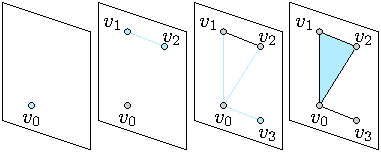
\includegraphics[scale=1.5]{simp_filt.pdf}
  \caption{\label{filtrationstack} Filtration of a simplicial complex showing the intermediate simplicial complex at each filtration step. A blue simplex indicates the simplex was added in that filtration step.}
\end{figure}

% (v_0,v_1,v_2,v_12,v_3,v_20,v_01,v_03,v_120)
% (1,2,2,2,3,3,3,3,4)
\end{example}

Algorithm 1 for a simplicial complex has, just like ordinary Gaussian elimination over fields, worst case time complexity $O(m^{3})$ where $m$ is the  number of simplices \cite{Zomorodian2005}. However, as seen in Example \ref{bddreduce} the boundary matrix is sparse. Furthermore, the decomposition of $H$ can be read entirely from the reduced boundary matrix without constructing an explicit presentation matrix. These are some areas where the algorithm usually is made more efficient, but dwelling on such optimizations is outside the scope of this thesis. For more in-depth treatments on this subject see  \cite{edels} for the theoretical underpinnings and \cite{ripser} for the de facto solution on which many software libraries are based.


\section{Visualizing Persistence}
The persistent homology of a space is not a very easy algebraic object to work with in practical terms. Even when considered under the bijection with intervals it is a multiset of intervals and as such helpful visualizations allow us to analyze and compare persistent homology. There are two principal ways of visualizing the decomposition of a persistence module: barcode diagrams and persistence diagrams.

\subsection{Barcodes}
A barcode diagram is a visual depiction of $B_{H}$ where each bar depicts the birth and death of a particular generator in one of the homology modules. The diagram gets its name from the way the intervals occur one after another which resembles a barcode.

In Figure \ref{annulus_barcode} we see a barcode diagram generated from points sampled from an annulus. Note that for small values of $\epsilon$ there are many generators of $H_{0}$, this is because the vertices have not been connected into a single component yet.

  We see that there some short intervals appearing for $H_{1}$ at around $\epsilon=0.3$ and we can see that these are not the hole that would represent the annulus, but rather noise that appears before $\epsilon$ has become large enough. At around $\epsilon=0.6$ the simplicial complex now captures the shape of the annulus and indeed the barcode diagram shows that we have one generator of $H_{0}$, the only connected component, and one generator of $H_{1}$ which is the hole in the middle of the annulus.

  Note how this hole in the middle of the annulus is gone when $\epsilon=1$ which highlights that it is difficult to find an optimal $\epsilon$.
\begin{figure}
  \centering
\begin{tikzpicture}
\node[inner sep=0pt] (barcode) at (0,0)
    {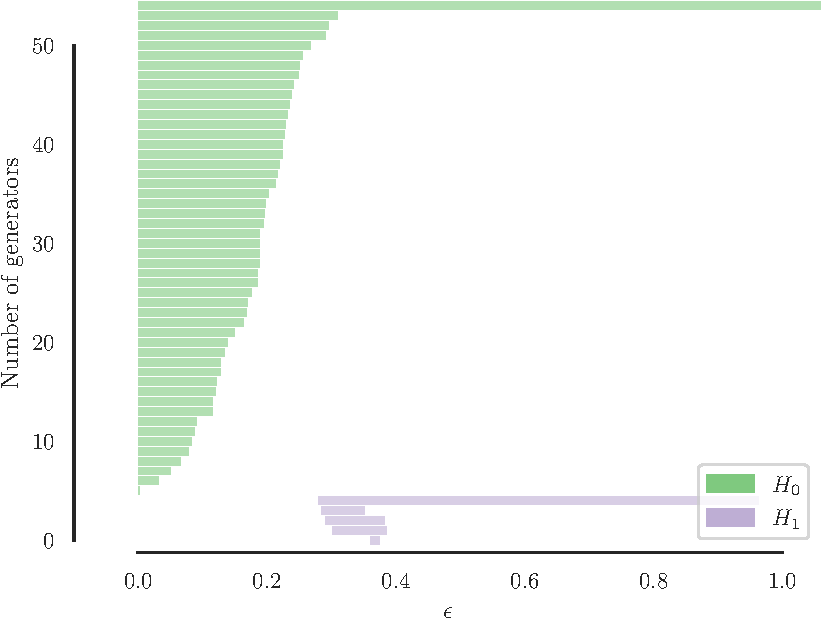
\includegraphics[scale=0.7]{barcode.pdf}};

\node[draw=black!100,line width=0.6mm, inner sep=0pt] (annulus0) at (-3.2,5.1)
    {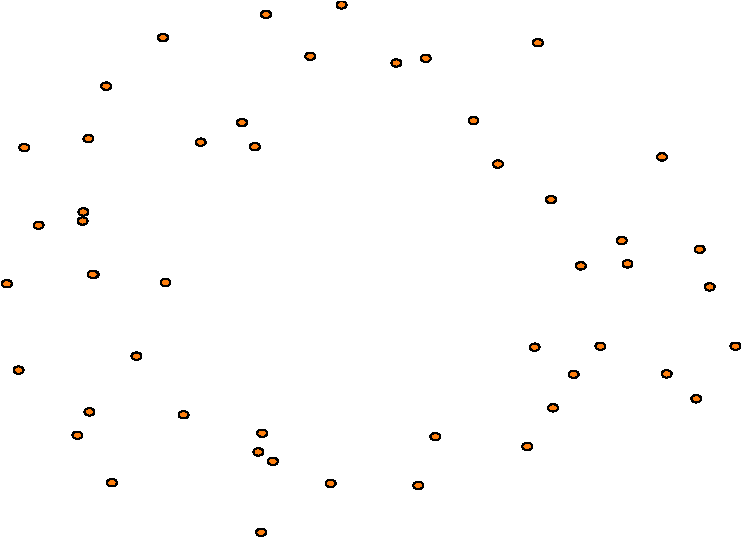
\includegraphics[scale=0.3]{annulus_eps0.pdf}};
    \draw[dotted,thick] (annulus0.south) -- (-3.2,-2.9);

\node[draw=black!100,line width=0.6mm, inner sep=0pt] (annulus3) at (-1,8)
    {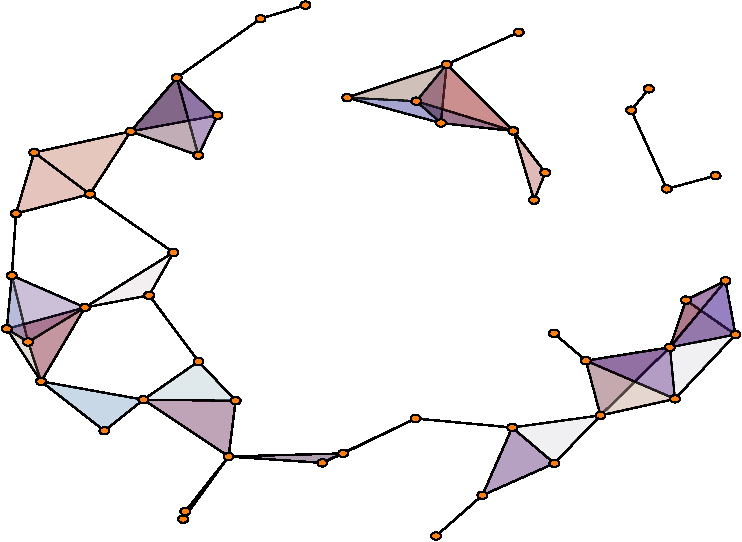
\includegraphics[scale=0.3]{annulus_eps3.pdf}};
\draw[dotted,thick] (annulus3.south) -- (-1,-2.9);

\node[draw=black!100,line width=0.6mm, inner sep=0pt] (annulus5) at (1.2,5.1)
    {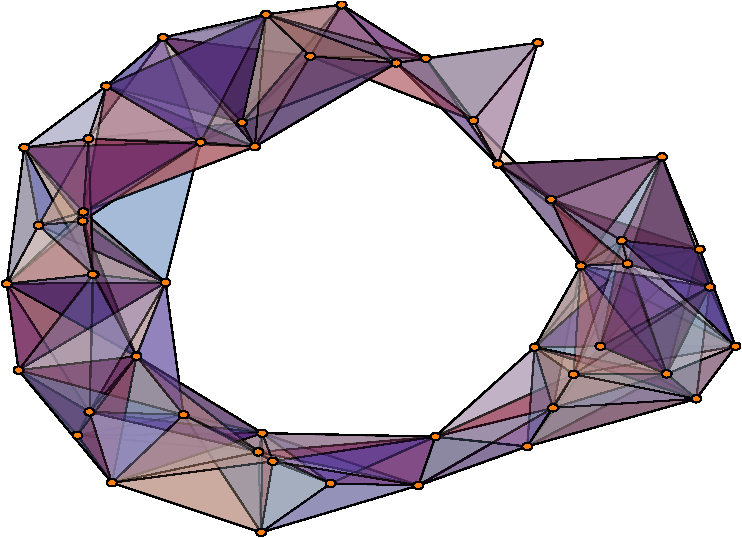
\includegraphics[scale=0.3]{annulus_eps5.pdf}};
    \draw[dotted,thick] (annulus5.south) -- (1.2,-2.9);
\node[draw=black!100,line width=0.6mm, inner sep=0pt] (annulus10) at (4.4,8)
    {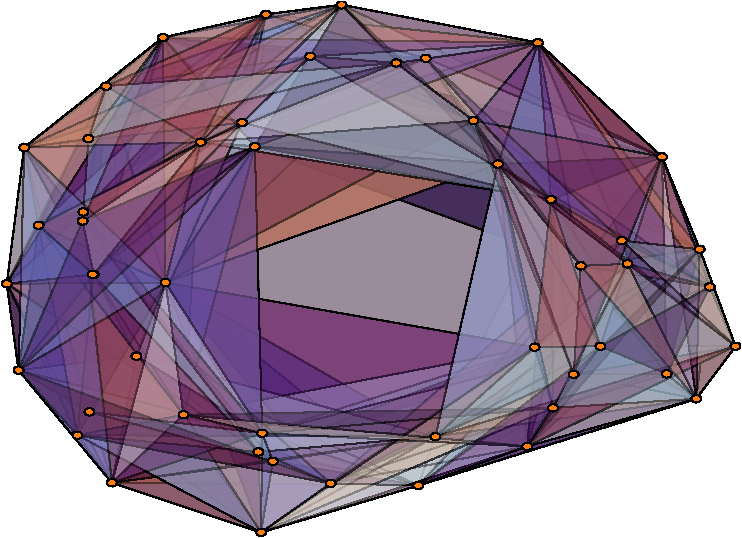
\includegraphics[scale=0.3]{annulus_eps10.pdf}};
\draw[dotted,thick] (annulus10.south) -- (4.4,-1.8);
\draw[dotted,thick] (4.4,-2.74) -- (4.4,-2.9);
\end{tikzpicture}
\caption{\label{annulus_barcode} Persistence barcode showing the birth and death of generators in the homology groups of a Vietoris-Rips complex approximated from points sampled from an annulus at different $\epsilon$. }
\end{figure}
  \subsection{Persistence Diagrams}
  Another way of illustrating persistent homology is the persistence diagram as seen in Figure \ref{pdiagram}.

  \begin{definition}
    The \textbf{persistence diagram} $X$ of a persistence module $M$ is a multiset of points in $\mathbb{R}^{2}\cup \{\infty\}$ defined as
    \[
      X:=\{ (x,y) \in \mathbb{R}^{2} \mid [x,y) \in \mathbf{B}_{M}\} \cup \{ (x,x) \mid | x \in \mathbb{R}\}.
    \]
  \end{definition}
In other words, it is the set of \textit{(birth,death)} pairs given by the intervals associated with the decomposition of $M$ together with all points on the diagonal.

When visualized as in Figure \ref{pdiagram} it serves alternative to the barcode in Figure \ref{annulus_barcode} where we instead plot the $\epsilon$-value on both axises and for each generator we draw a point given by its corresponding interval. When we have a lot of intervals this is a preferable way of visualizing the persistent homology, since unlike the barcode it does not grow vertically with the number of intervals. Generators that never die are mapped at a line representing infinity.

Just like in the barcode in Figure \ref{annulus_barcode} we can see in Figure \ref{pdiagram} that the only two generators that live for a considerable amount of time is a single connected component in $H_{0}$ and a single hole in $H_{1}$. This is consistent with the topology that we expect from an annulus. At around $\epsilon=0$ we see a lot of $H_{0}$ generators being born and dying at almost the same time. Since the number of generators of $H_{0}$ tells us the number of connected components in the topology this clearly illustrates how the sampled points go from being isolated islands to being incorporated in a larger simplex.
\begin{figure}[ht]
  \centering
  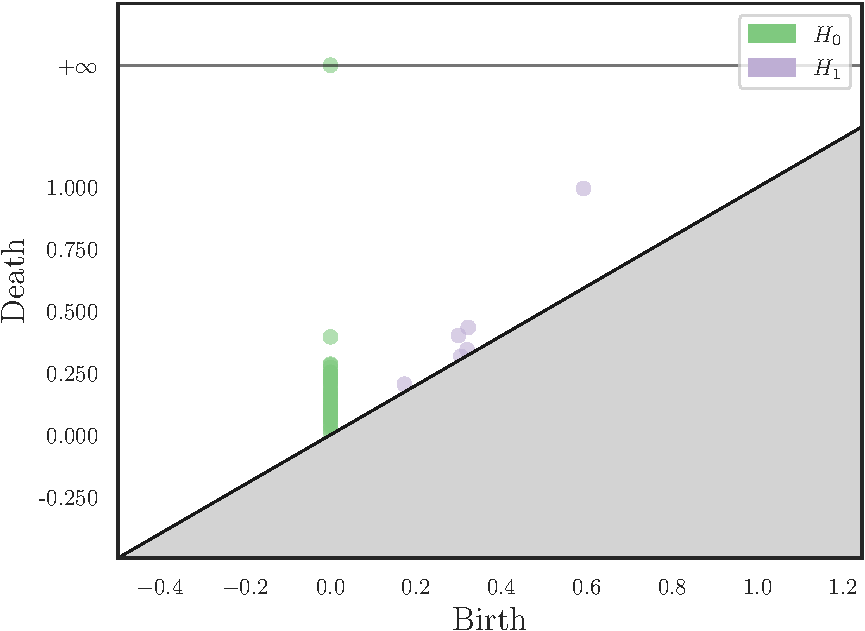
\includegraphics[scale=0.7]{diagram.pdf}
  \caption{\label{pdiagram} A persistence diagram over the birth and death of generators in the homology groups of a Vietoris-Rips complex approximated from points sampled from an annulus. The closer a point is to the diagonal line the shorter it lived. }
\end{figure}

  \section{Metrics}
  As persistent homology is often used as a topological summary of some data, it can be benefitial to be able to compare two different data samples with respect to their persistent homology. There are two commonly used metrics for doing this, the bottleneck distance and the Wasserstein distance.
  \begin{definition}
    The \textbf{bottleneck distance} between two persistence diagrams $X,Y$ is
    \[W_{\infty}(X,Y) = \inf_{\beta: X \to Y} \sup_{x \in X} ||x-\beta(x)||_{\infty}\]
    where $\beta$ is a bijection from $X$ to $Y$.
  \end{definition}
In other words, the bottleneck distance finds a matching, in the space of possible matchings, between the two persistence diagrams such that the largest distance in the matching is the smallest one possible. Since there could be more intervals in one persistence diagram, any point can also be matched with an infinite number of points on the diagonal which are included in the persistence diagram. Its name is derived from the fact that there is only one matching of points which contributes to the actual value of the distance, the largest one, and hence the distance is ``bottlenecked'' by that matching.

One disadvantage of the bottleneck distance is that it is quite coarse, it does not tell us very much about the other distances between other matched points. An alternative is the $q$-Wasserstein distance which instead incorporates all distances in the best matching.
  \begin{definition}
    The q-Wasserstein distance between two persistence diagrams $X,Y$ is
    \[W_{q}(X,Y) = (\inf_{\beta: X \to Y} \sum_{x \in X}  ||x-\beta(x)||_{\infty}^{q})^{\frac{1}{q}}\]
  \end{definition}
  Both the Wasserstein and bottleneck distance have their role as the bottleneck distance can be considered more robust to noise, since small changes in the matchings are ignored in favor of the largest matching.

  A desired quality of these metrics are stability, ideally we want the metrics to actually reflect difference in the underlying spaces. There are stability theorems that under varying conditions fulfill a meta-theorem which guarantee this.

  \begin{definition}
    A filtration function $X \to \mathbb{R}$ is a function from a simplicial or cubical complex $X$ such that the sublevel set $\{ f^{-1}(a,\infty) \mid a \in \mathbb{R} \}$ is a filtration.
  \end{definition}

  \begin{theorem}[Stability meta-theorem \cite{vejdemo}]\label{stab}
    For a nice enough space $X$ and nice enough filtration functions $f,g: X \to \mathbb{R}$, a nice enough norm of the difference of $f-g$ serves as an upper bound to the distances between the persistence diagrams given by $f,g$.
  \end{theorem}

  In other words, a small perturbation of the filtering functions will at most be as large as the difference between the functions themselves. The term \textit{nice} is intentionally vague, since these conditions vary. For an overview of the particular scenarios in which the meta-theorem is applicable see \cite{vejdemo}, including a formulation which allows for general persistence modules under certain conditions. In our practical applications we are only considering finitely many sublevel sets from a filtration function which motivates the following definition.

  \begin{definition}
    A filtration is called \textbf{tame} if the persistence complex arising from the filtration function is of finite type.
  \end{definition}

Then we have the following corollary of the meta-theorem.

  \begin{corollary}\label{stabtame}
    If $f,g$ given as in Theorem \ref{stab} are \textit{tame} then the meta-theorem holds for the bottleneck distance with norm given by the $L_{\infty}$-norm and for the $q$-Wasserstein distance with the $L_{q}$-norm.
  \end{corollary}
  As the proofs of Corollary \ref{stabtame} require a lot of tedious and technical details which would detract from the overall theme of this thesis, we instead refer the reader to elementary proofs regarding the $q$-Wasserstein distance in \cite{skraba2021wasserstein} and the bottleneck distance in \cite{skraba2021notes}.
%%% Local Variables:
%%% mode: latex
%%% TeX-master: "thesis.tex"
%%% End:
